\documentclass[11pt,a4paper]{article}

% -------------------------------------------------
% Pacchetti
% -------------------------------------------------
\usepackage[margin=2.5cm]{geometry}
\usepackage{amsmath,amssymb}
\usepackage{siunitx}
\usepackage{graphicx}
\usepackage{microtype} % aiuta a ridurre Overfull/Underfull hbox
\usepackage{caption}
\usepackage{subcaption}
\usepackage{hyperref}

% Impostazioni didascalie: evita righe troppo piene
\captionsetup{format=plain,justification=raggedright,singlelinecheck=false}

\title{Hover Disc a 20\,cm: Approccio Energetico con Cuscino Centrale e Getto di Corona}
\author{}
\date{\today}

\begin{document}
\maketitle

\section{Schema e dominio di calcolo}

\begin{figure}[ht]
  \centering
  % usa \linewidth per evitare overfull dei float larghi
  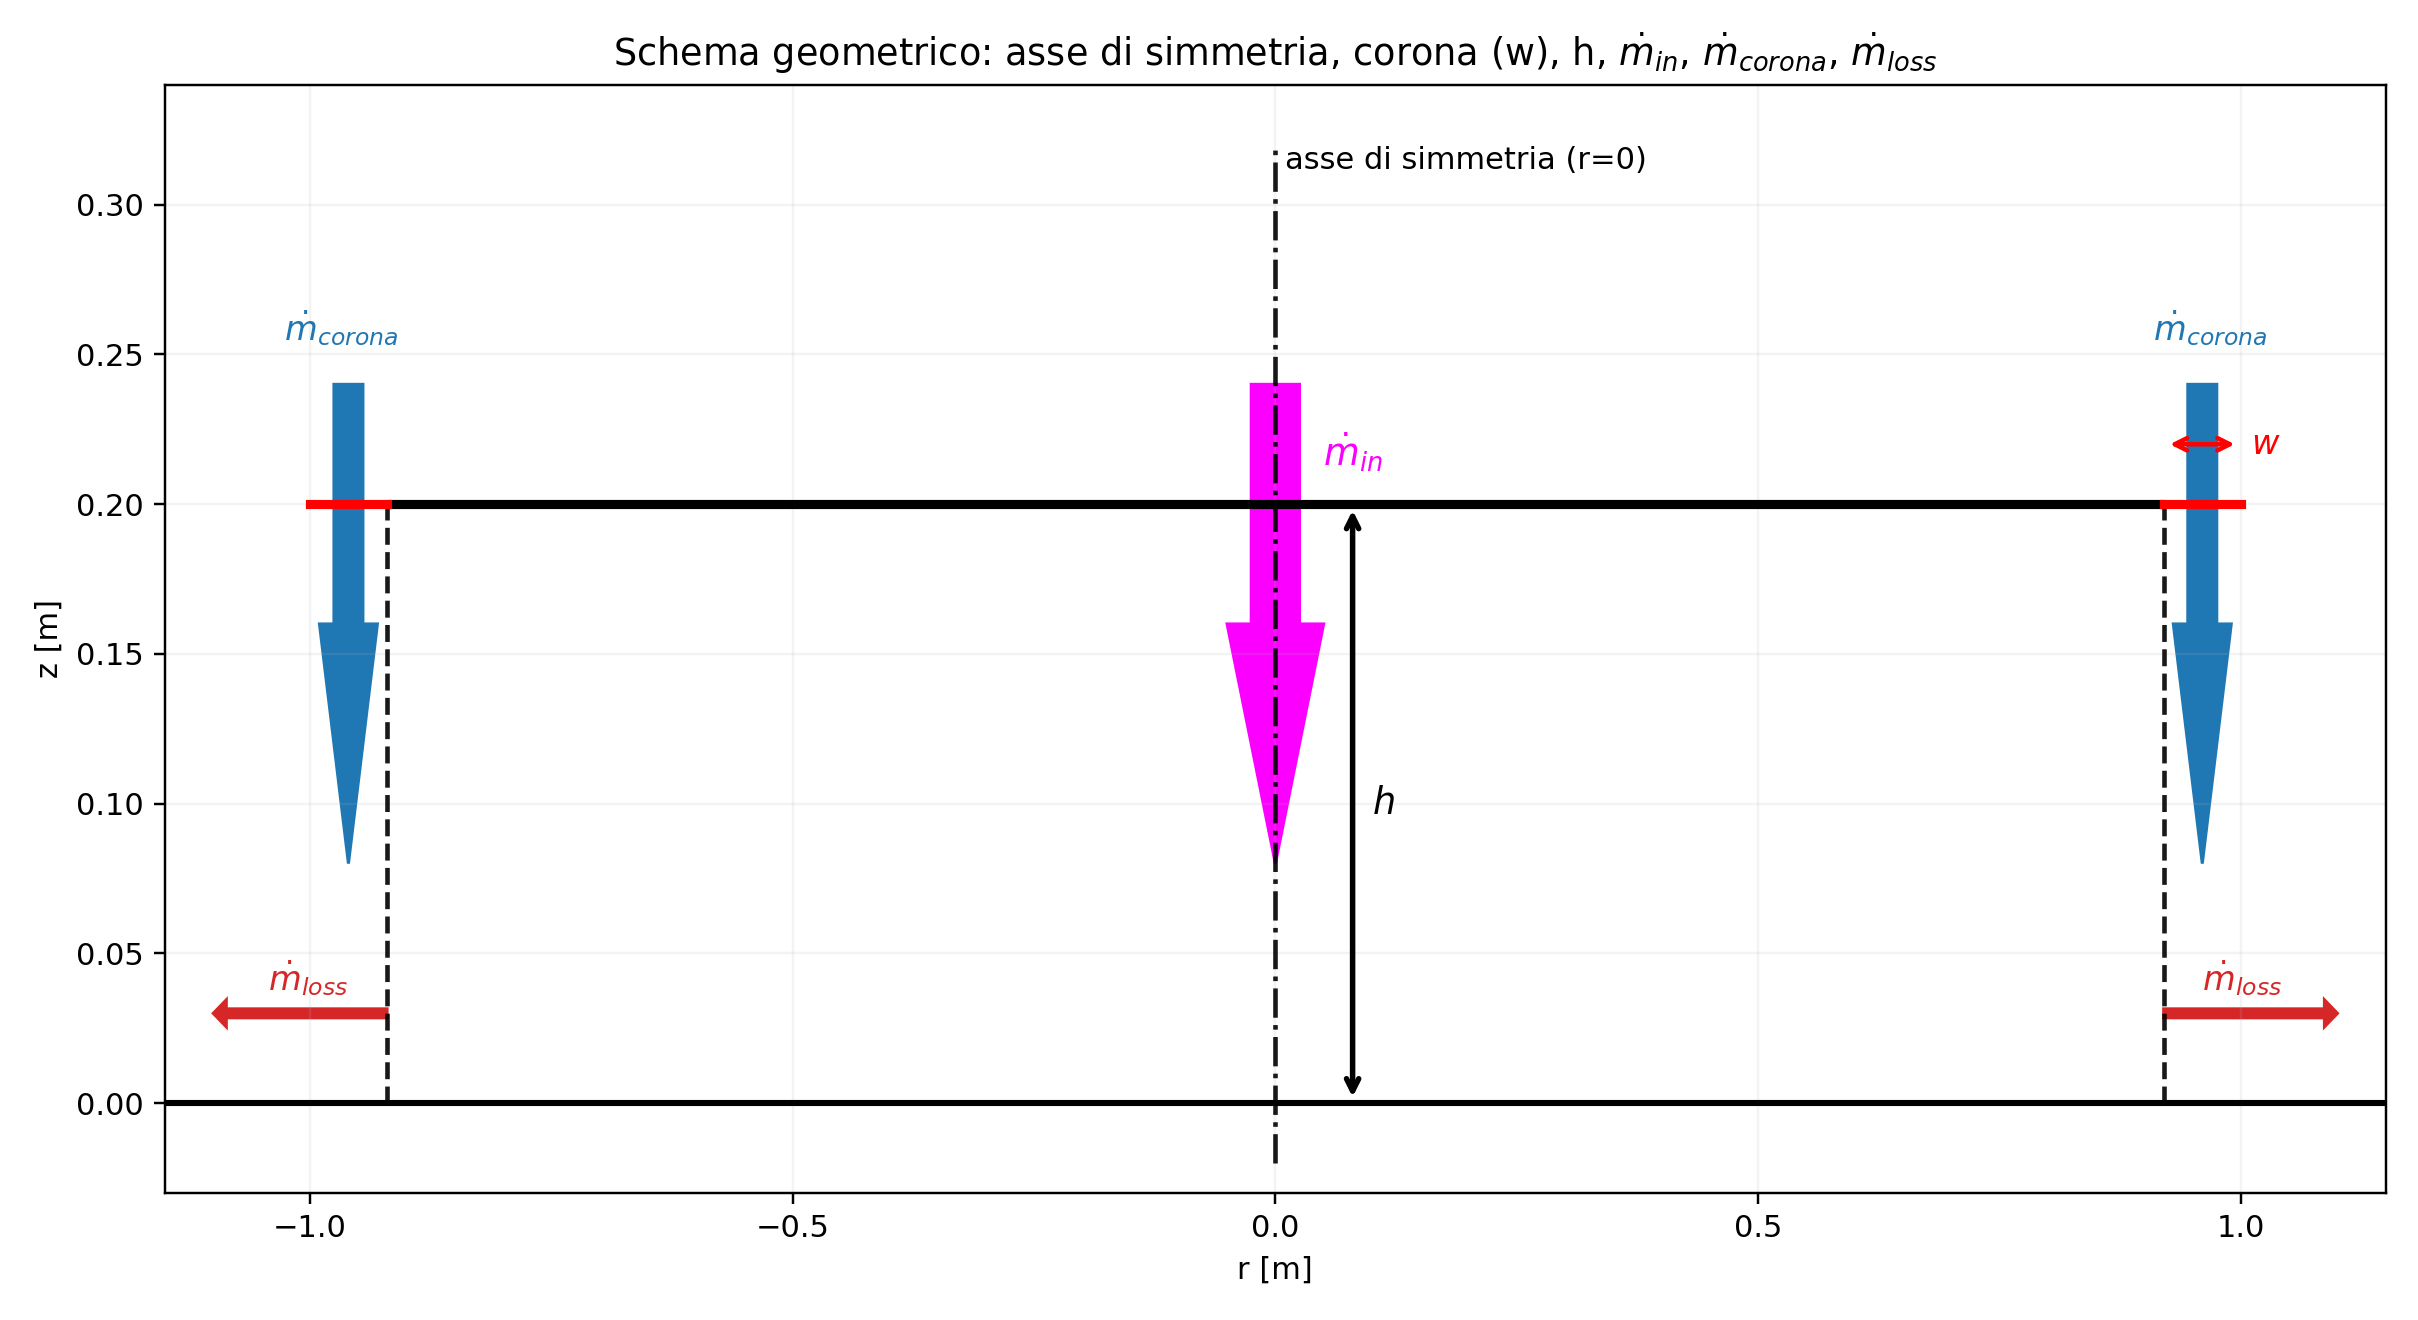
\includegraphics[width=0.8\linewidth]{./figures/schema_geometry.png}
  % Evita math in PDF strings con \texorpdfstring
  \caption{Schema assi-simmetrico: disco sospeso a quota \texorpdfstring{$h$}{h}, zona centrale
  \texorpdfstring{$0\le r\le R_i$}{0≤r≤Ri} a pressione quasi uniforme \texorpdfstring{$p_c$}{pc}, corona periferica di larghezza
  \texorpdfstring{$w$}{w} con getto radiale, portata entrante \texorpdfstring{$\dot{m}_{\mathrm{in}}$}{mdot\_in}, portata della corona
  \texorpdfstring{$\dot{m}_{\mathrm{corona}}$}{mdot\_corona} e dispersione laterale
  \texorpdfstring{$\dot{m}_{\mathrm{loss}}$}{mdot\_loss}. Per simmetria assiale si può considerare metà dominio.}
  \label{fig:schemageo}
\end{figure}

Il problema viene posto in termini energetici: determinare quanta potenza minima deve essere fornita per mantenere il disco a distanza \(\,h\) dal suolo con una pressione imposta \(\,p_c\) nella regione centrale
\(\,0\le r\le R_i,\,0\le z\le h\), mentre i lati sono aperti (assenza di pareti rigide o skirt) e l'unico confinamento laterale è garantito dal getto di \emph{corona} che agisce come air--curtain. Indichiamo con \(R_{\mathrm{tot}}\) il raggio esterno, con \(w\) la larghezza della corona e con \(R_i=R_{\mathrm{tot}}-w\) il raggio interno del cuscino portante.

\section{Pressione imposta e baseline energetica}
La portanza è fornita dall'area centrale \(A_c=\pi R_i^2\). La pressione richiesta per sostenere un carico utile \(m\) è
\begin{equation}
  p_c=\frac{m g}{A_c}=\frac{m g}{\pi R_i^2}.
\end{equation}
La baseline energetica del cuscino è la potenza di flusso di pressione che entra nell'area a \(p_c\):
\begin{equation}
  P_{\mathrm{cuscino}}^{\min}=p_c\,Q_{\mathrm{in}}=p_c\,\frac{\dot{m}_{\mathrm{in}}}{\rho}.
\end{equation}
Tutto il resto (getti, miscelazione, turbolenza, inefficienze meccaniche/elettriche) si somma a questa baseline.

\section{Fuga laterale con air--curtain e altezza efficace \texorpdfstring{$h_{\mathrm{out}}$}{h\_out}}

Con i lati aperti, l'aria esce radialmente alla periferia. Il getto di corona riduce l'\emph{apertura efficace} di fuga da \(h\) ad un valore \(h_{\mathrm{out}}<h\), grazie alla propria quantità di moto. Un criterio ingegneristico per legare \(h_{\mathrm{out}}\) ai parametri del curtain (fessura \(t\), velocità del getto \(V_{\mathrm{jet}}\)) è un bilancio di quantità di moto per unità di circonferenza:
\begin{equation}
  \rho\,V_{\mathrm{jet}}^2\,t \;\gtrsim\; \kappa\,p_c\,h_{\mathrm{out}},
  \qquad \Rightarrow \qquad
  h_{\mathrm{out}}\;\approx\;\frac{\rho\,V_{\mathrm{jet}}^2\,t}{\kappa\,p_c},
  \label{eq:hout}
\end{equation}
con \(\kappa=\mathcal{O}(1)\) che ingloba dettagli geometrici (angolo del getto, aderenza/Coandă, turbolenza).

La fuga laterale \(Q_{\mathrm{loss}}\) (quindi \(\dot{m}_{\mathrm{loss}}=\rho\,Q_{\mathrm{loss}}\)) si può modellare con due regimi, scegliendo in base al numero di Reynolds nel gap.

\paragraph{Regime orifizio (inerziale).}
Valido per \(Re\gg 2000\) nel varco al bordo:
\begin{equation}
  A_e=2\pi R_{\mathrm{tot}}\,h_{\mathrm{out}},\qquad
  Q_{\mathrm{loss}}=C_d\,A_e\,\sqrt{\frac{2p_c}{\rho}},
  \qquad
  P_{\mathrm{cuscino}}^{\min}=p_c\,Q_{\mathrm{loss}}.
\end{equation}

\paragraph{Regime di lubrificazione (viscoso).}
Valido per gap piccoli e \(Re\) basso (fuga radiale tra piastre distanti \(h_{\mathrm{out}}\)):
\begin{equation}
  Q_{\mathrm{loss}}=\frac{\pi\,h_{\mathrm{out}}^3\,p_c}{6\,\mu\,\ln\!\left(\tfrac{R_{\mathrm{tot}}}{R_i}\right)},
  \qquad
  P_{\mathrm{cuscino}}^{\min}=p_c\,Q_{\mathrm{loss}}.
\end{equation}

\section{Costo energetico del curtain}
La corona è un getto anulare a raggio \(R_i\) con fessura \(t\). La sua portata e potenza cinetica (ideale) sono:
\begin{equation}
  \dot{m}_{\mathrm{corona}}=\rho\,(2\pi R_i\,t)\,V_{\mathrm{jet}},
  \qquad
  P_{\mathrm{jet}}=\tfrac{1}{2}\,\dot{m}_{\mathrm{corona}}\,V_{\mathrm{jet}}^2.
\end{equation}
L'air--curtain \emph{non} entra nel bilancio di massa della regione centrale (che resta \(\dot{m}_{\mathrm{in}}=\dot{m}_{\mathrm{loss}}\)), ma determina \(h_{\mathrm{out}}\) via \eqref{eq:hout} e quindi abbassa \(Q_{\mathrm{loss}}\) e \(P_{\mathrm{cuscino}}^{\min}\).

\section{Potenza totale minima e criterio di regime}
La potenza minima ideale di sistema (fluido) è la somma:
\begin{equation}
  P_{\mathrm{tot}}^{\min}=P_{\mathrm{cuscino}}^{\min}+P_{\mathrm{jet}}.
\end{equation}
Per scegliere il modello di perdita, usiamo \(Re=\tfrac{\rho U h_{\mathrm{out}}}{\mu}\) con una stima della velocità caratteristica \(U\) al bordo:
\[
\text{se }Re\gg 2000 \ \Rightarrow\ \text{orifizio (inerziale)},\qquad
\text{altrimenti}\ \Rightarrow\ \text{lubrificazione (viscoso)}.
\]
La potenza elettrica reale richiederà \(P_{\mathrm{elettrica}}\approx P_{\mathrm{tot}}^{\min}/\eta\) con \(\eta\) efficienza globale (ventilatori, condotti, driver).

\section{Procedura rapida di progetto}
\begin{enumerate}
  \item Fissa \(R_{\mathrm{tot}}, R_i\) (quindi \(w\)), \(h\), \(m\) \(\Rightarrow\) calcola \(p_c\).
  \item Scegli \(t\) e \(V_{\mathrm{jet}}\) \(\Rightarrow\) calcola \(h_{\mathrm{out}}\) con \eqref{eq:hout}.
  \item Seleziona il regime (Re) e calcola \(Q_{\mathrm{loss}}(h_{\mathrm{out}})\) \(\Rightarrow\)
        \(P_{\mathrm{cuscino}}^{\min}=p_c\,Q_{\mathrm{loss}}\).
  \item Calcola \(\dot{m}_{\mathrm{corona}}, P_{\mathrm{jet}}\) \(\Rightarrow\) \(P_{\mathrm{tot}}^{\min}\).
  \item Ottimizza \(t, V_{\mathrm{jet}}, w\) per minimizzare \(P_{\mathrm{tot}}^{\min}\) garantendo \(h_{\mathrm{out}}\ll h\).
\end{enumerate}

\section{Esempio numerico (ordine di grandezza)}
Sia \(R_{\mathrm{tot}}=\SI{1.00}{m}\), \(w=\SI{0.05}{m}\) \(\Rightarrow R_i=\SI{0.95}{m}\); \(h=\SI{0.20}{m}\); \(m=\SI{40}{kg}\).
Aria: \(\rho=\SI{1.2}{kg/m^3}\), \(\mu=\SI{1.8e-5}{Pa\,s}\).
Corona: \(t=\SI{1.0}{mm}\), \(V_{\mathrm{jet}}=\SI{60}{m/s}\), \(\kappa=1.3\), \(C_d=0.65\).
\[
A_c=\pi R_i^2=\SI{2.835}{m^2},\quad
p_c=\frac{mg}{A_c}\approx \SI{138}{Pa}.
\]
\[
h_{\mathrm{out}}\approx\frac{\rho V_{\mathrm{jet}}^2 t}{\kappa p_c}
\approx \SI{0.024}{m}.
\]
\[
A_e=2\pi R_{\mathrm{tot}} h_{\mathrm{out}}\approx \SI{0.151}{m^2},\quad
Q_{\mathrm{loss}}=C_d A_e\sqrt{\tfrac{2p_c}{\rho}}\approx \SI{1.50}{m^3/s}.
\]
\[
P_{\mathrm{cuscino}}^{\min}=p_c Q_{\mathrm{loss}}\approx \SI{0.21}{kW}.
\]
\[
\dot{m}_{\mathrm{corona}}=\rho (2\pi R_i t) V_{\mathrm{jet}}\approx \SI{0.43}{kg/s},\quad
P_{\mathrm{jet}}=\tfrac12 \dot{m}_{\mathrm{corona}} V_{\mathrm{jet}}^2\approx \SI{0.77}{kW}.
\]
\[
P_{\mathrm{tot}}^{\min}\approx \SI{0.98}{kW}\quad(\text{fluido, ideale}).
\]
Con efficienza complessiva \(\eta\in[0.5,0.65]\), attesi \(\sim \SI{1.5}{kW} - \SI{2.0}{kW}\) elettrici.

\end{document}
